% results_fit.tex
\subsection{Model Fit and Diagnostics}

\texttt{sfa()} runs the whole pipeline in one call; automatic retention
chose five factors, fixed as \texttt{nfactors~=~5}, and the warning
confirms the keying-free encoding ignores the scoring column.

{\scriptsize
\begin{verbatim}
> fit_auto <- sfa(big5_df, embeddings = E8, encoding = "mean_centered_pearson")
Warning message:
'scoring' has reverse-keyed items but is ignored for encoding =
"mean_centered_pearson": this method is keying-free by design. Use
"atomic_reversed" for keyed sign-flipping.
> cat("Auto-retained factors:", fit_auto$factors, "\n")
Auto-retained factors: 5
> fit <- sfa(big5_df, embeddings = E8, encoding = "mean_centered_pearson",
+            nfactors = 5)
> fit
Semantic Factor Analysis
  Encoding: mean_centered_pearson
  Embedding dim: 4096
  Factors:5 (minres + oblimin)

Diagnostics:
  KMO:  0.971 (marvelous - higher is better)
  TEFI: -27.7059 (lower is better)
  RMSR: 0.0323 (good - lower is better)
  CAF:  0.4120 (marginal - higher is better)

[item-by-factor loadings omitted; reported in full in the supplement]

                 MR3   MR1   MR2   MR5   MR4
SS loadings    6.421 5.330 4.111 3.193 2.736
Proportion Var 0.128 0.107 0.082 0.064 0.055
Cumulative Var 0.128 0.235 0.317 0.381 0.436

Factor correlations (Phi):
      MR3   MR1   MR2   MR5   MR4
MR3 1.000 0.685 0.606 0.577 0.539
MR1 0.685 1.000 0.538 0.582 0.555
MR2 0.606 0.538 1.000 0.465 0.446
MR5 0.577 0.582 0.465 1.000 0.398
MR4 0.539 0.555 0.446 0.398 1.000
\end{verbatim}
}

KMO was .971, RMSR .032, TEFI $-27.71$, and CAF .412; substantial factor
correlations ($\phi = .40$--$.69$) again reflect the similarities'
shared positive component. \texttt{summary(fit)} adds the per-factor
McDonald's omegas:

{\scriptsize
\begin{verbatim}
McDonald's omega per factor:
 factor omega_assigned omega_theoretical matched_theoretical
    MR3          0.908             0.902         Neuroticism
    MR1          0.863             0.850   Conscientiousness
    MR2          0.830             0.560       Agreeableness
    MR5          0.709             0.583        Extraversion
    MR4          0.704             0.732            Openness
\end{verbatim}
}

The solution recovers the Big Five: Neuroticism anchors MR3,
Conscientiousness MR1, Openness MR4; MR2 and MR5 split Agreeableness and
Extraversion items into warmth/other-orientation and gregariousness
factors (Figure~\ref{fig:loadings};
Table~\ref{tab:s-semantic-loadings}). Communalities ranged from .566
(A23) to .905 (N16); the assigned--theoretical omega gaps---MR2 .830
vs.\ .560, MR5 .709 vs.\ .583---quantify this mixing: internally
coherent factors that cross the theoretical boundary.

\begin{figure}[H]
\centering
\captionsetup{justification=raggedright,singlelinecheck=false}
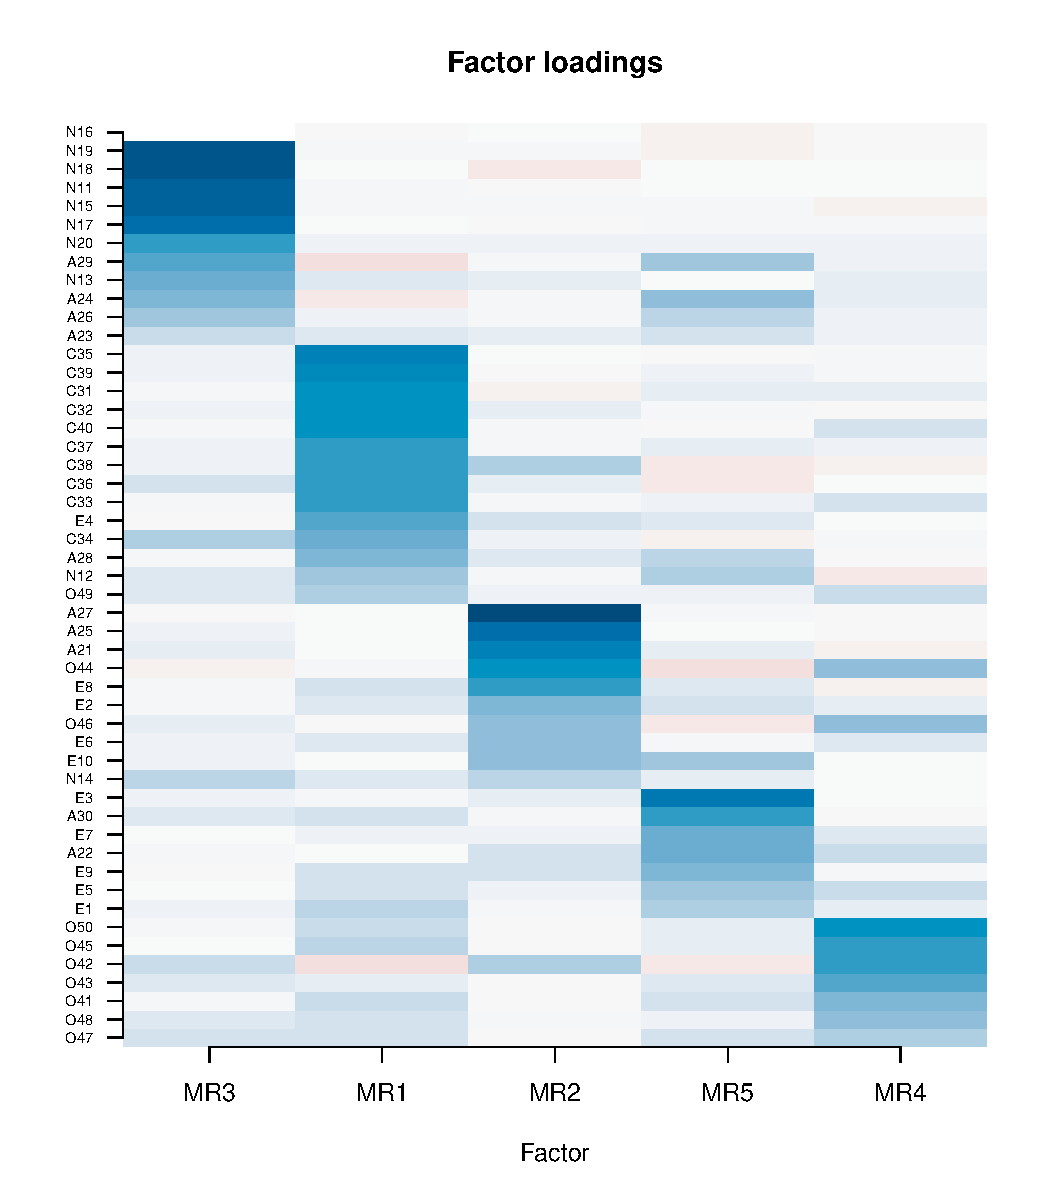
\includegraphics[width=0.6\textwidth]{figures/loadings.pdf}
\caption{Item-by-factor loading heatmap for the five-factor semantic
solution, produced by \texttt{plot(fit, type = "loadings")}. Items are
sorted by their dominant factor; MR3 = Neuroticism, MR1 =
Conscientiousness, MR2 and MR5 = Agreeableness/Extraversion blends, MR4 =
Openness.}
\label{fig:loadings}
\end{figure}

Conventional thresholds need not transfer to embedding-derived matrices
\citep{pokropek-2026}, so \texttt{calibrate~=~TRUE} draws Monte~Carlo reference distributions for
RMSR, CAF, and TEFI from data-matched null embeddings (100 replicates,
54.7~s):

{\scriptsize
\begin{verbatim}
> fit_cal <- sfa(big5_df, embeddings = E8, encoding = "mean_centered_pearson",
+                nfactors = 5, calibrate = TRUE, calibrate_iter = 100)
> cat("calibrate=TRUE elapsed:", round(t_cal["elapsed"], 1), "s\n")
calibrate=TRUE elapsed: 54.7 s
> fit_cal$calibration
[lists of 100 null RMSR, CAF, and TEFI values; omitted]
\end{verbatim}
}

Across the 100 nulls, RMSR ranged from .0119 to .0134, CAF from .501 to
.532, and TEFI from $-21.66$ to $-17.82$; the observed TEFI ($-27.71$)
undercut every null---a more entropically organized five-factor
partition---while the observed RMSR (.032) and CAF (.412) fell above and
below their ranges: the real similarities carry residual structure beyond
five factors that nulls lack, an index-by-index recalibration that raw
thresholds would obscure. \texttt{as\_psych(fit)} lets
\texttt{psych::fa.sort()} and \texttt{psych::factor.congruence()} treat
the fit like a response-based solution.
